\section{UAV and deployment unit}\label{sec:DeploymentUnit(UAV)}

The UAV is a custom-built, 177 cm wingspan hexacopter, controlled by a Pixhawk flight controller running ArduPilot Mega flight software. The UAV has a 3DR GPS module using the UBlox NEO-7 chipset.


 The deployment mechanism allows the UAV to carry four SeismicDarts in a circular array, and release them when it reaches the desired GPS location, one at a time.
 The rear of the dart has a circular tip that locks into the deployment mechanism, and rests on a rectangular slot-path. 
 A servomotor rotates the dart tips through the rectangular slot-path, allowing darts to release from a circular opening,  as shown in Fig.~\ref{fig:deployment_system}.



\begin{figure} \centering
  {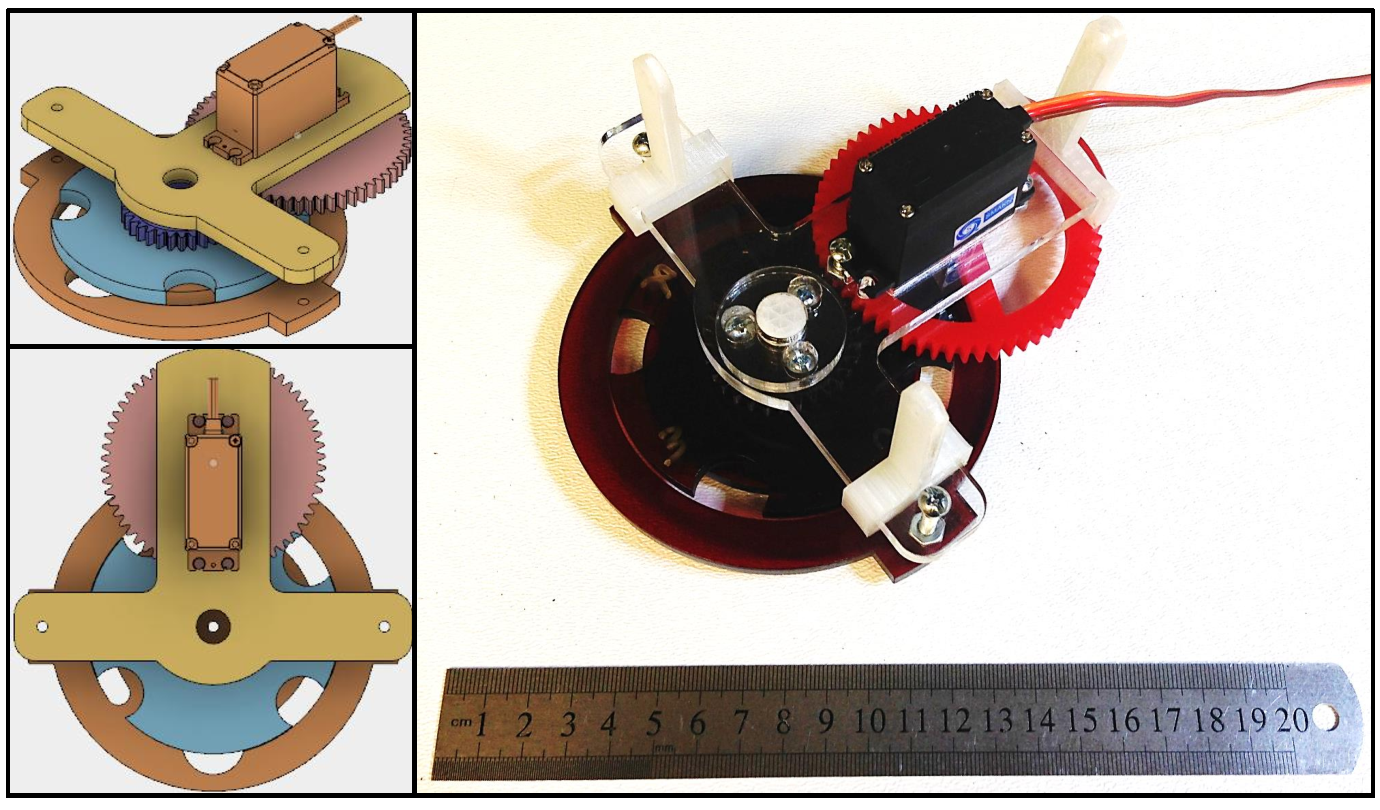
\includegraphics[width=\columnwidth]{deployment_system.pdf}}
 \caption{Deployment system for dropping SeismicDarts from the UAV. Pictured design holds 4 darts, but can be scaled according to the UAV's carrying capacity.} 
 \label{fig:deployment_system}
\end{figure}




\subsection{Autonomous drop demonstration and accuracy}

The current UAV can place the SeismicDart within $\pm1$ m of the desired location.  
This range is within tolerances for seismic surveys because:
(1) often features (rocks, water, etc.) exist that require this amount of error from theoretically assigned locations,
(2) some survey designs include a random placement component to improve noise cancellation.
%(3) this error minimally perturbs the data since seismic waves travel at 600 m/s near the surface, so a one-meter inaccuracy equates to $\approx$1.6 ms delay.
%(4) the response of a receiver to seismic vibrations is an average over a number of meters.  ?? what does this mean??

The critical factor is to know within $\approx$10 cm accuracy the geophone location.  Such accuracy can be obtained through Real Time Kinematic GPS systems. Knowledge of the exact location compensates for placement inaccuracy.
%allows corrections for jitter in signal arrival times due to  placement inaccuracy.


%Exp 4: Automatic drop from drone, accuracy in placement
\begin{figure} \centering
  {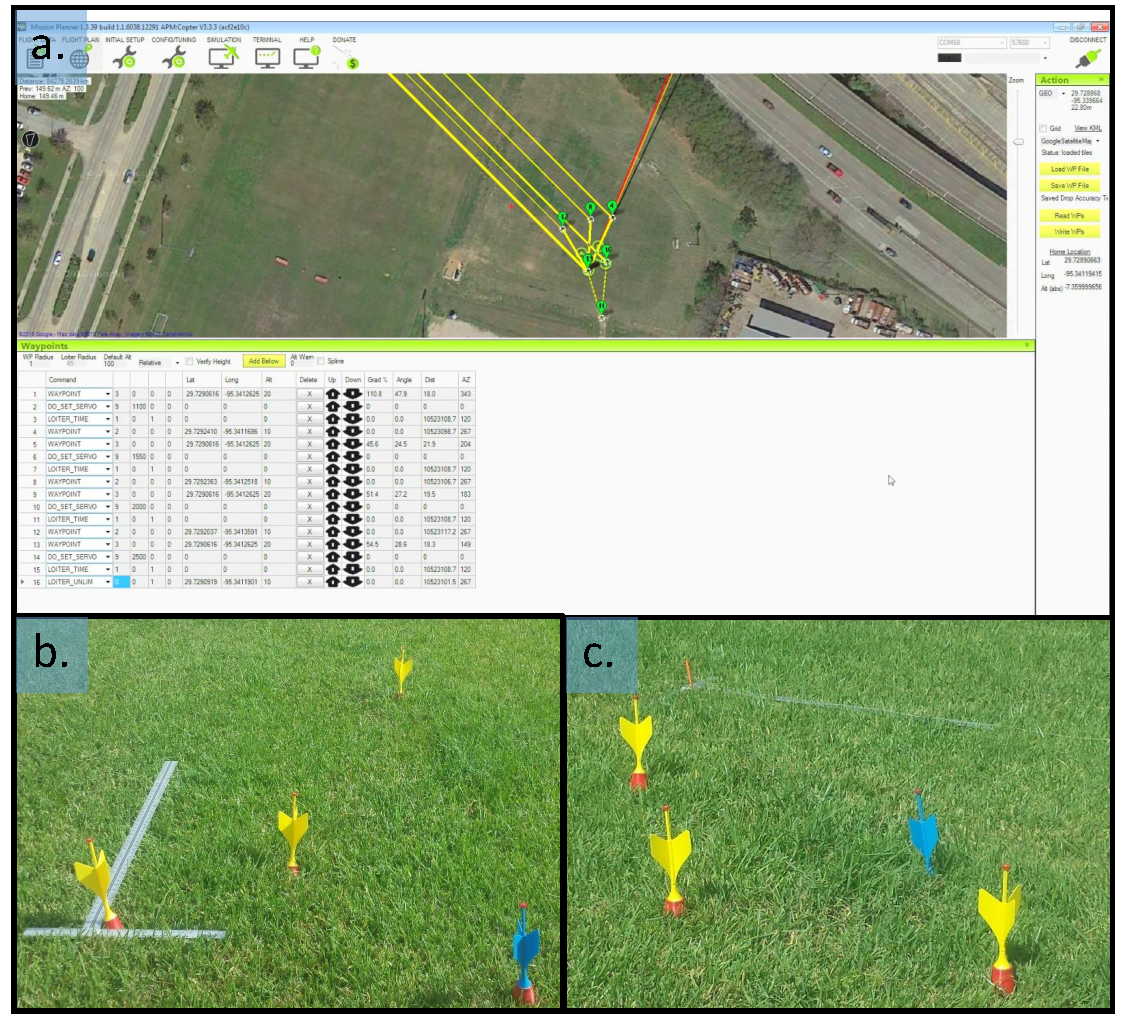
\includegraphics[width=\columnwidth]{accuracy_test_overview.pdf}}
 \caption{a.) Flight plan of accuracy test. b.) First set of darts with reference axes. c.) Third dart set. } 
 \label{fig:Accu_test_darts}
\end{figure}

For the accuracy test, six sets of darts, four darts in each set, were dropped on the same GPS waypoint. Between each drop, the UAV travelled to a nearby GPS waypoint to cancel out the flight controller's stable hover.  This path is shown in Fig.~\ref{fig:Accu_test_darts}a. The UAV then returned to the launch platform to be reloaded and data was recorded after each set.

To record data, one dart was picked from the first set as the reference point (the lower left in Fig.~\ref{fig:Accu_test_darts}b), hence the first data point was (0,0). A 1-m T-square was placed with the origin at the dart's drop point to establish reference axes.

After the first set of data was recorded, the darts were collected and reloaded on the UAV for the next deployment set.
 A rod was placed in the position of the first dart to keep reference as shown in Fig.~\ref{fig:Accu_test_darts}c. 
 The T-square was kept in place and mason twine was suspended to lengthen the reference axes. 
 Future deployments were measured  using the reference point and axes. 
  Results are shown in Fig.~\ref{fig:SD_accu.pdf}.


\begin{figure} \centering
  {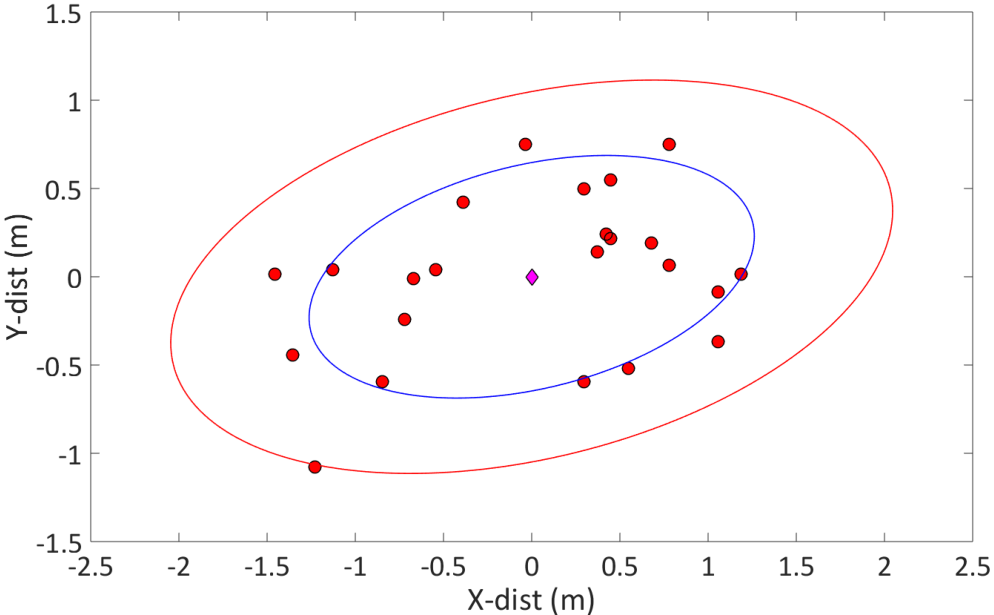
\includegraphics[width=\columnwidth]{SD_accu.pdf}}
 \caption{Landing locations of 24 darts, each commanded to drop at the same GPS location. 
 \label{fig:SD_accu.pdf}}
\end{figure}


\subsection{Height vs. penetration depth}
%Exp 5: Height vs. penetration depth

FAA rules require that UAVs fly below 400 feet (122 m). Our highest drop tests were from 20 m, and resulted in well-planted geophones on a grass field with density 3.3 kg/cm$^3$. Harder soils may require faster impact velocity, so this section examines possible impact velocities as a function of drop height.
For ease of analysis we will assume the SeismicDart has a constant coefficient of drag $C_d$ and that the drag force is proportional to velocity squared and equal to $\frac{1}{2} v^2 \rho A C_d$, where $v$ is the velocity, $A$ the cross-sectional area and $\rho$ the density of air.  
 The tests were performed near sea level, so $\rho \approx 1.225  \text{kg/m}^3$.
  The dart body is 0.06 m in diameter so $A=0.028$ m$^2$.  We will assume the dart $C_d$ is between that of a streamlined body $C_d=0.04$ and that of an arrow $C_d=1.5$~\cite{miyazaki2013aerodynamic}, and choose that of a sphere $C_d=0.47$.
The terminal velocity is then
\begin{align}
v_T = \sqrt{\frac{2 m g}{\rho A  C_d}} \approx 59 \text{ m/s.}
\end{align}
The velocity at impact is a function of the drop height $h$.
\begin{align}
v_{impact} = v_T  \sqrt{ 1 - e^{ -\frac{\rho A  C_d}{m} h }} \approx 59\sqrt{ 1 - e^{ -0.008 h }} \text{ m/s}
\end{align}
With  $C_d=0.47$, our drop from 20m achieves only 38\% the terminal velocity (19.0 m/s), and for $C_d=0.04$ only 12\% terminal velocity  (19.7 m/s).
%This implies our tests are far from the limits of the SeismicDart's per
This implies the SeismicDart is suitable even for much harder soils than tested thus far.

%\begin{figure} \centering
%  {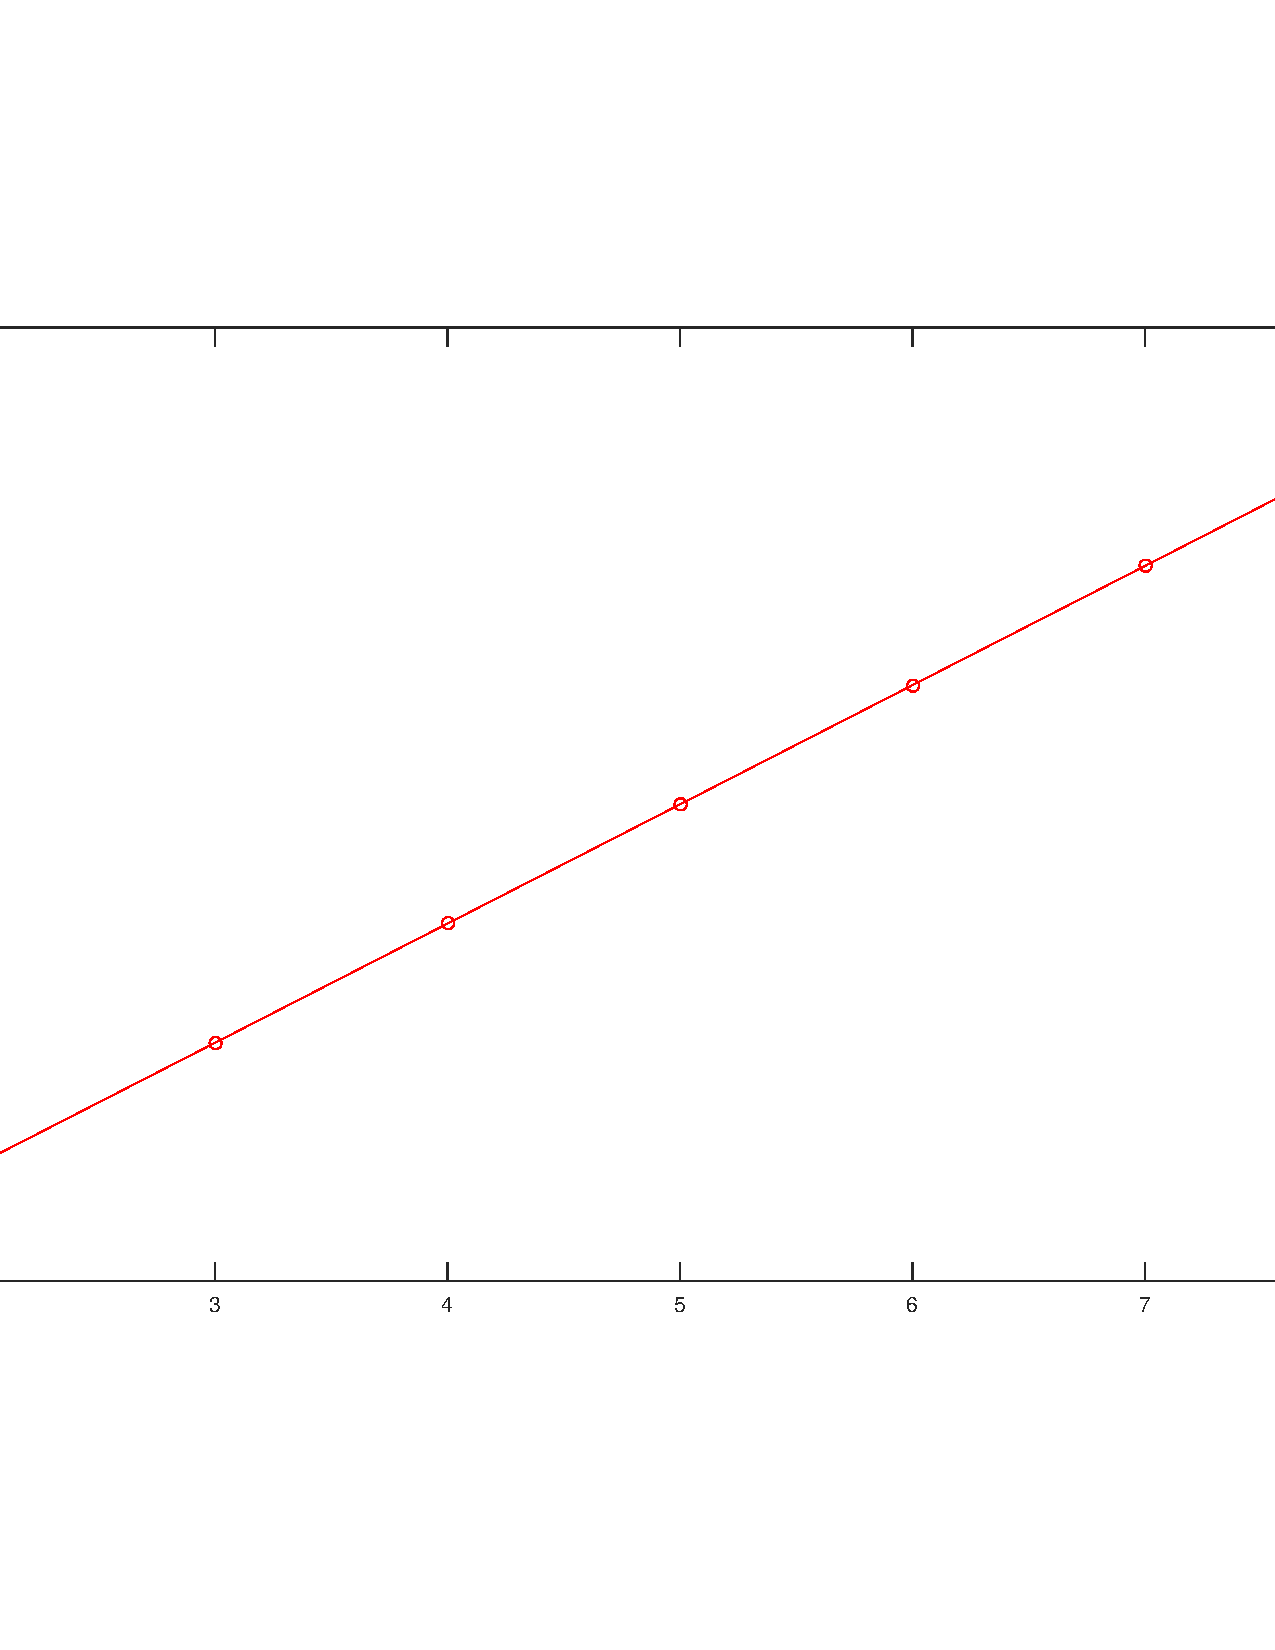
\includegraphics[width=\columnwidth]{replace_graph.pdf}}
% \caption{Plot of pneumatic cannon firing angle vs ending angle} 
% \label{fig:TradvsAutoDrop}
%\end{figure}





